\RequirePackage{luatex85}
\documentclass{standalone}

% Default preamble
\usepackage{pgfplots}
\usepackage{tikz}
\usetikzlibrary{%
    patterns, plotmarks, backgrounds, shapes, arrows, calc, trees, positioning,
    chains, shapes.geometric, decorations.pathreplacing,
    decorations.pathmorphing, shapes.arrows, decorations.markings, quotes,
    arrows.meta, spy, fit, matrix, math
}

% Custom preamble from global variable:
\usetikzlibrary{patterns}
\usepackage{xcolor}
\definecolor{efm1}{HTML}{017EC3}
\definecolor{efm2}{HTML}{F31E26}
\definecolor{efm3}{HTML}{019E5E}
\definecolor{efm4}{HTML}{FBA61D}
\definecolor{efm5}{HTML}{916237}

\usepackage{graphicx}
\usepackage{caption}
\usepackage{subcaption}
\usepackage{amsmath}

\renewcommand{\familydefault}{\sfdefault}

\begin{document}

\begin{figure}
    \begin{tikzpicture}
        \node[start] () {
\includegraphics[]{../03-remove-borders/remove-borders.pdf}};
        \node[font=\large,xshift=-3.25cm,yshift=0.9cm] () {oaa[m]};
        \node[font=\large,xshift=-1.9cm,yshift=1.2cm] () {asp[m]};
        \node[font=\large,xshift=-0.4cm,yshift=1.2cm] () {asp[c]};
        \node[font=\large,xshift=1.0cm,yshift=-0.65cm] () {oaa[c]};
        \node[font=\large,xshift=2.10cm,yshift=1.75cm] () {mal[m]};
        \node[font=\large,xshift=3.05cm,yshift=-0.65cm] () {mal[c]};
        \node[font=\large,xshift=-1.9cm,yshift=-0.65cm] () {cit[m]};
        \node[font=\large,xshift=-0.4cm,yshift=-0.65cm] () {cit[c]};
        \node[font=\large,xshift=-3.25cm,yshift=-1.65cm] () {glu[c]};
        \node[font=\large,xshift=3.15cm,yshift=-1.80cm] () {glu[m]};
        \node[font=\large,xshift=-1.85cm,yshift=-2.95cm] () {akg[m]};
        \node[font=\large,xshift=1.0cm,yshift=-2.95cm] () {akg[c]};

        \node[rectangle,xshift=-4.5cm,yshift=-4.6cm,minimum width=0.5cm,minimum height=0.5cm,fill=efm1,draw=black] (P1) {};
        \node[font=\large,right=0.1cm of P1] (E1) {AEFM 1.};
        \node[rectangle,minimum width=0.5cm,minimum height=0.5cm,fill=efm2,draw=black,right=0.1cm of E1] (P2) {};
        \node[font=\large,right=0.1cm of P2] (E2) {AEFM 2.};
        \node[rectangle,minimum width=0.5cm,minimum height=0.5cm,fill=efm3,draw=black,below=0.1cm of P1] (P3) {};
        \node[font=\large,right=0.1cm of P3] (E3) {AEFM 3.};
        \node[rectangle,minimum width=0.5cm,minimum height=0.5cm,fill=efm4,draw=black,right=0.1cm of E3] (P4) {};
        \node[font=\large,right=0.1cm of P4] (E4) {AEFM 4.};
        \node[rectangle,minimum width=0.5cm,minimum height=0.5cm,fill=efm5,draw=black,below=0.1cm of P3] (P5) {};
        \node[font=\large,right=0.1cm of P5] (E5) {AEFM 5.};
        \node[font=\large,xshift=2.5cm,yshift=-5.2cm] () {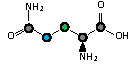
\includegraphics[width=4cm]{../../../../../source-metabolite-structures/glutamine-carbon-3-4.pdf}};
    \end{tikzpicture}
\end{figure}

\end{document}

